\documentclass{article}

\begin{document}

\begin{verbatim}
124 Latex
=========

124.0 Texgestaltung
-------------------
Hier wird erklärt, wie du Texte formatierst.

Beachte

kleiner- und größergeschriebenen Text,
Zeilenumbrüche
Leerzeilen
Farben

Der Lesefluss innerhalb eines Artikels sollte nicht durch hervorgehobene
Textelemente gestört werden.

124.0.1 Reference
..................
https://de.wikipedia.org/wiki/Hilfe:Textgestaltung#Formatierungen,_die_nicht_in_Wikipedia-Artikeln_verwendet_werden_sollten

124.0.2 Example
................
xxx


124.1 Piktogramm
----------------

124.1.1 Definition
..................
Ein Piktogramm ist ein Symbol, das einen Hinweis durch ein einfaches Bild vermittelt.
Siehe: https://de.wikipedia.org/wiki/Piktogramm.

124.1.2 Referenz
................
https://de.answacode.com/tex/441917/gibt-es-eine-einfache-moglichkeit-strichmannchen-in-pgftikz-zeichnungen-zu-verwe
https://ftp.rrze.uni-erlangen.de/ctan/graphics/pgf/contrib/tikzsymbols/tikzsymbols.pdf

124.1.3 Strichmännchen
......................
The package provides various emoticons, cooking symbols and trees:

\usepackage{tikzsymbols}

\begin{document}
    \begin{tikzpicture}
    \Strichmaxerl[3]
    \end{tikzpicture}
\end{document}

124.1.4 Emoticon
................
\dSmiley [2][yellow]


124.2 Latex Color
-----------------
The color package also supports decimal values in the RGB color model that
accepts integer values in the interval [0,255].

124.2.1 Inet address
....................
https://latexcolor.com/

124.2.2 Definition
...................
\usepackage[dvipsnames]{xcolor}          % Using the color package

\definecolor{amethyst}{rgb}{0.6, 0.4, 0.8}

124.2.3 Example
...............
{\color{red} Erziehung}


124.3 Zeichnen mit Tikz
-----------------------

124.3.1 Kurs
............
Wir wollen in diesem Vortrag aufzeigen, wie simple Zeichnungen, aber auch
Graphen, Bäume und Diagramme durch wenige einfache Befehle direkt aus einem
LaTeX-Dokument heraus gesetzt werden können:
https://www.mlte.de/latex/tikz-talk/

124.3.2 Basic Drawing
.....................
In this first post we'll start with the basics, showing how to draw simple
shapes, with subsequent posts introducing some of the interesting things you
can do using the tikz package:
https://de.overleaf.com/learn/latex/LaTeX_Graphics_using_TikZ%3A_A_Tutorial_for_Beginners_(Part_1)%E2%80%94Basic_Drawing

124.3.3 Chemie
..............
https://www.latex-kurs.de/kurse/WS2017/FK2/Druck_FK2_Tikz.pdf

124.3.4 Examples
................
https://texample.net/tikz/examples/

124.3.5 Arrows
..............
This post is about exploring TikZ arrows in LaTeX provided by the arrows.meta
library. We will learn how to change the arrow tip (head), the arrow thickness,
the arrow color and add arrow label.   

https://latexdraw.com/exploring-tikz-arrows/

124.3.6 Rectangular shape with a border
.......................................
Could anyone please tell me how do I draw a rectangular shape with a black border around it?

https://tex.stackexchange.com/questions/105876/drawing-a-rectangular-shape-with-a-border-around-it-in-tikz

124.3.7 Stacked coloured underlines
...................................
Stacking of objects:
https://ftp.agdsn.de/pub/mirrors/latex/dante/macros/latex/contrib/stackengine/stackengine.pdf
\usepackage{stackengine}

Overlapping highlighting:

https://tex.stackexchange.com/questions/169189/highlighting-text-through-stacked-colored-underlines


124.4 Counter
-------------
124.4.1 Similar Problem
........................
I would like to create a custom counter:
https://tex.stackexchange.com/questions/326258/create-custom-counter

124.4.2 Transfer
................
% Subparagraph counter.
\newcounter{subParagraphC}
\renewcommand{\thesubParagraphC}{\bf\arabic{subParagraphC}.}

% Begin of a subparagraph
\newcommand\subParagraph[1] {%
  \stepcounter{subParagraphC}
  \bf{\theparagraph}\thesubParagraphC \hskip 6pt \rm #1
}

% Description counter.
\newcommand\desccount{%
  \stepcounter{subParagraphC}\theparagraph\thesubParagraphC
}


124.5 Command with two arguments
--------------------------------
see
https://www.tutorialspoint.com/tex_commands/newcommand.htm

\newcommand - Used to create your own commands (control sequences, macros,
definitions).

124.2 Synopsis
..............
{ \newcommand\myCommandName
  [ <optional # of arguments, from 1 to 9> ]
  { <replacement text> } }
  
124.2 Description
.................
\newcommand command is used for defining your own commands ...

124.5 Example
.............
\documentclass{article}
\usepackage{soul}  % Provides letter spacing, underlining, striking out, etc.
\newcommand{\xx}[2]{ arg1: ,,\st{#1}''; args: ,,{\large #2}'' }
\begin{document}
test: \xx{first}{second}
\end{document}


124.6 TikZ: adding text
-----------------------

124.6.1 Reference
.................
https://tex.stackexchange.com/questions/29233/tikz-adding-text#comment57371_29233

124.6.2 Description
...................
In TikZ you can use nodes to place almost anything (in particular, text) in the
position you want.

124.6.3 Example
...............
\documentclass{article}
\usepackage{tikz}
\begin{document}
\tikz {\node[draw,align=left] at (3,0) {x \\y \\ z};}
\end{document}


124.7 TikZ: memoving bounding box of text node
----------------------------------------------

124.7.1 Reference
.................
https://tex.stackexchange.com/questions/170645/removing-bounding-box-of-text-node-tikz

124.7.2 Description
...................
The draw key in the options list for the node tells TikZ to draw the node shape
around the node. And the default node shape is rectangle.
Remove the draw key from the node options to not draw the node.

124.7.3 Example
...............
\documentclass{article}
\usepackage{tikz}
\begin{document}
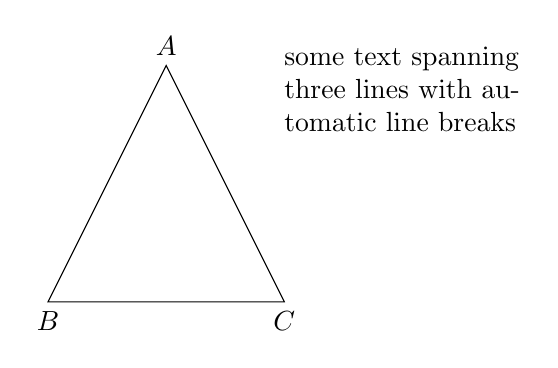
\begin{tikzpicture}
  \draw (0, 1.3) node[below] {$B$} -- (3, 1.3) node[below] {$C$} -- 
    (1.5, 4.3) node[above] {$A$} -- cycle;
  \node[text width=3cm] at (4.5,4) 
    {some text spanning three lines with automatic line breaks};
\end{tikzpicture}
\end{document}


124.8 TikZ: tuturial
--------------------

124.8.1 Reference
.................
https://www.mit.edu/afs.new/sipb/project/latex/tutorial_latex_tikz.pdf
https://ctan.org/pkg/pgf

124.8.2 Description
...................
What ist TikZ?
PGF: protable graphics format
Allows creation of vetocr graphic schemes

124.8.3 Drawing a path
......................
\documentclass{article}
\usepackage{tikz}
\begin{document}
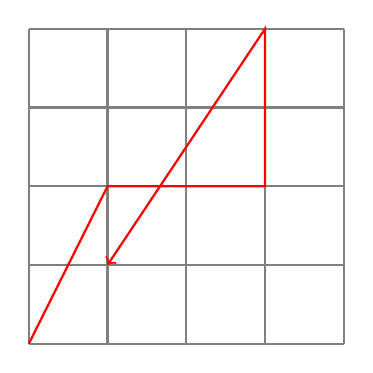
\begin{tikzpicture}
  \draw[help lines, thick] (0,0) grid (4,4);
  \draw[->, thick, red] (0,0) -- (1,2) -| (3,4) -- (1,1);
\end{tikzpicture}
\end{document}


124.9 TikZ: style
-----------------
PGF is a macro package for creating graphics:
create PostScript and PDF graphics in TEX.

124.9.1 Reference
.................
https://de.wikipedia.org/wiki/PGF/TikZ
https://ctan.org/pkg/pgf
https://tex.stackexchange.com/questions/34719/tikz-style-attribute-for-adding-default-node-text
https://www.overleaf.com/learn/latex/LaTeX_Graphics_using_TikZ%3A_A_Tutorial_for_Beginners_(Part_3)%E2%80%94Creating_Flowcharts

124.9.2 Description
...................
“What is TikZ?” Basically, it just defines a number of TEX commands
that draw graphics.
see
https://ctan.mirror.norbert-ruehl.de/graphics/pgf/base/doc/pgfmanual.pdf


124.9.3 Example
...............
\documentclass{article}
\usepackage{tikz}
\begin{document}
 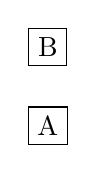
\begin{tikzpicture}[%
  stuff/.style={%
    draw,
    node contents={A}} ]
\node at (0,0) [stuff];
\node at (0,1) [stuff, node contents={B}];
\end{tikzpicture}
\end{document}


124.9 Emacs: Schriftgröße
-------------------------

124.9.1 Reference
.................
https://de.answacode.com/stackoverflow/5533110/emacs-vergrossernverkleinern

124.9.2 Beschreibung
....................
Nach einer Kombination (C-x C-+ oder C-x C--), aufeinanderfolgend + oder -
erhöhen oder verringern Sie den Textmaßstab, ohne C-x C- erneut zu tippen.


124.10 TikZ: filled rectangle without border
--------------------------------------------
The border of the rectangle is drawn because you are using the \draw command,
which, by definition, draws the specified path (here the rectangle). The fact
that you are adding the option fill=orange just tells TikZ that in addition it
should fill the path with orange. Replacing \draw with \fill will do what you
are expecting.

124.10.1 Reference
..................
https://tex.stackexchange.com/questions/82530/how-to-draw-a-filled-rectangle-without-a-border-using-tikz

124.10.2 Example
................
\documentclass{article}
\usepackage{tikz}
\begin{document}
\tikz \fill [orange] (0.1,0.1) rectangle (1,1);
\end{document}


124.11 Euro symbol
------------------

124.11.1 Reference
..................
https://tex.stackexchange.com/questions/9866/latest-advice-on-the-euro-symbol

124.11.2 Example
................
\documentclass{article}
\usepackage{eurosym}
\begin{document}
10€ and 10\euro
\let\texteuro\euro
10€ and 10\euro
\end{document}


124.12 Tikz: draw a vertical
----------------------------

124.12.1 Reference
..................
https://tex.stackexchange.com/questions/402454/tikz-draw-a-vertical-line-to-a-straight-line

124.12.2 Example
................
\documentclass{article}
\usepackage{tikz}
\begin{document}
\tikz { \draw [line width=1pt, -] (0, 0) -- (0, 1); }
\end{document}


124.13 Minipage
---------------
Minipage is an environment to produce parboxes in LaTeX. 

124.13.1 Reference
..................
https://latex-tutorial.com/minipage-latex/

124.13.2 Example
................
\documentclass{article}
\begin{document}
\begin{minipage}{6cm}
  This text is processed in paragraph mode, and then becomes an indivisible
  \TeX{} box.
\end{minipage}
\end{document}


124.14 Nahsinne, Fernsinne
--------------------------
Nahsinne, Sinnesorgane der Haut und der Geschmackssinn im Gegensatz zu den
Fernsinnen (Sehen, Hören und Geruch) (Sinne).

Weitere Sinne beim Menschen
Die moderne Sinnesphysiologie kennt für den Menschen klassischerweise noch vier
weitere Sinne:

Temperatursinn, Thermorezeption
Schmerzempfindung, Nozizeption
Vestibulärer Sinn, Gleichgewichtssinn
Körperempfindung, Tiefensensibilität.

Dazu gehören:
Lage- und Bewegungssinn, Propriozeption
Organsinne, Viszero- oder Enterozeption (unter anderem empfunden als Hunger,
Durst oder Harndrang)

124.15.1 Reference
..................
https://www.spektrum.de/lexikon/psychologie/nahsinne/10283
https://de.wikipedia.org/wiki/Sinn_(Wahrnehmung)


124.16 Römische Zahlen
----------------------
Schreibweise mit Vinculum

Ein Vinculum (auch Titulus) ist ein Querstrich über den Ziffern.

124.16.1 Reference
..................
https://golatex.de/viewtopic.php?t=3886
https://de.wikipedia.org/wiki/R%C3%B6mische_Zahlschrift

124.16.2 Example
................
\documentclass{article}
\usepackage{amsmath}
\newcommand{\rom}[1]{$\underline{\overline{\text{#1}}}$}
\begin{document}
In diesem Text werden die zwei r\"omischen Zahlen \rom{XII} und \rom{IV}
dargestellt.
\end{document}


124.17 Auflistung mit Punkten
-----------------------------

124.17.1 Reference
..................
https://latex-kurs.blogspot.com/2012/12/latex-aufzahlungen.html

124.17.2 Example
................
\documentclass{article}
\begin{document}
\begin{itemize}
\item 1 
\item 2
\end{itemize}
\end{document}


124.18 Space between the itemize "items"
----------------------------------------

124.18.1 Reference
..................
https://tex.stackexchange.com/questions/12373/how-to-change-the-space-between-the-itemize-items-in-latex

124.18.2 Example
................
\documentclass{article}
\begin{document}
X
\begin{itemize}
  \setlength\itemsep{0em}
\item 1 
\end{itemize}
\end{document}

\documentclass{article}
\usepackage{enumitem}
\begin{document}
\noindent No spacing between this line and the item list below it.
\begin{itemize}[noitemsep,topsep=0pt]
    \setlength\itemsep{0em}
  \item Item 1
  \item Item 2
  \item Item 3
\end{itemize}
\end{document}


124.19 Horizontal spacing
-------------------------

124.19.1 Reference
..................
https://tex.stackexchange.com/questions/74353/what-commands-are-there-for-horizontal-spacing

124.19.2 Example
................


124.20 Underlining with dash-dotted line
----------------------------------------

124.20.1 Reference
..................
https://tex.stackexchange.com/questions/327972/underlining-with-dash-dotted-line
https://ftp.gwdg.de/pub/ctan/graphics/pgf/base/doc/pgfmanual.pdf, p. 166

124.20.2 Example
................
\documentclass{article}
\usepackage{tikz}
\newcommand{\mydash}[1]{%
  \tikz[baseline=(dashed.base)]{
    \node[inner sep=1pt, outer sep=0pt] (dashed) {#1};
    \draw[dashed, line width=1.5pt, color=magenta]
    ([yshift=-2pt]dashed.south west) -- ([yshift=-2pt]dashed.south east);
    }%
}%
\begin{document}
\mydash{dashed line}
\end{document}

\end{verbatim}
\end{document}
